\chapter{Preparation}
% Principally, this chapter should describe the work which was undertaken before code was written, hardware built or theories worked on. It should show how the project proposal was further refined and clarified, so that the Implementation stage could go smoothly rather than by trial and error.
% Throughout this chapter and indeed the whole dissertation, it is essential to demonstrate that a proper professional approach was employed.
% The nature of this chapter will vary greatly from one dissertation to another but, underlining the professional approach, this chapter will very likely include a section headed “Requirements Analysis” and incorporate other references to software engineering techniques.
% The chapter will cite any new programming languages and systems which had to be learnt and will mention complicated theories or algorithms which required understanding.
% It is essential to declare the Starting Point (see Section 7). This states any existing codebase or materials that your project builds on. The text here can commonly be identical to the text in your proposal, but it may enlarge on it or report variations. For instance, the true starting point may have turned out to be different from that declared in the proposal and such discrepancies must be explained.

%  ~2,500 words


This chapter presents in more depth the brain age estimation problem (Section~\ref{brain-age-estimation}) and the dataset used for the brain age estimation task (Section~\ref{dataset}). It also gives background on population graphs (Section~\ref{population-graphs}) as well as the neural network architectures for implementing them (Sections~\ref{training-gcn} and~\ref{training-gat}).

\section{Brain age estimation}
\label{brain-age-estimation}

The \textit{brain age} is defined as the \textit{apparent} age of the brain, compared to the person's true (or \textit{chronological}) age. For example, a highly atrophied brain of a young person may appear to have a higher brain age than a healthy brain of an older person, because gradual atrophy is related to the normal brain ageing process. 

Formally, the brain age $y_b$ can be expressed as the sum of the known chronological age $y_c$ and the unknown \textit{brain age gap} $\varepsilon_g$ that is defined as the discrepancy between the chronological and the brain age~\cite{niu2019improved}:

\begin{equation}
    \label{brainage:eq1}
    y_b = y_c + \varepsilon_g.
\end{equation}

It is generally assumed~\cite{franke2019ten} that a typical healthy person has a normally ageing brain, so the brain age corresponds to chronological age:

\begin{equation}
    \label{brainage:assume}
    y_b \approx y_c.
\end{equation}

Our goal is to estimate brain age $y_b$ as a function $f$ of brain imaging features $X$:

\begin{equation}
    \label{brainage:eq2}
    y_b = f(X) + \varepsilon_e,
\end{equation}

where $\varepsilon_e$ is the prediction error, while the estimate of \textit{chronological} age is instead (from Equations~\eqref{brainage:eq1} and~\eqref{brainage:eq2})

\begin{align}
    y_c &= f(X) + \varepsilon,
        \label{brainage:eq3}
\end{align}

where $\varepsilon \coloneqq \varepsilon_e - \varepsilon_g$ is the error term consisting of both the brain age gap and the model prediction error.

Since the brain age $y_b$ is unknown, any (semi-)supervised machine learning model can only use chronological age as predicted variable, following Equation~\eqref{brainage:eq3}. However, if the model is trained on healthy subjects only, $f(\cdot)$ can explain both the apparent brain age \textit{and} the chronological age with $X$, since for healthy subjects $y_b \approx y_c$ (Equation~\eqref{brainage:assume}) and any variance in $\varepsilon$ is assumed to contain just the prediction error $\varepsilon_e$. When the same model is applied to non-healthy subjects, $f(\cdot)$ explains the chronological age assuming the brain is healthy, and any \textit{additional} unexplained variance in $\varepsilon$ is assumed to be the brain age gap. On the other hand, if the model is trained on both healthy and non-healthy subjects at the same time, it might learn the combined confounding effects of both normal (chronological) and disease-related (brain) ageing, thus hiding the brain age gaps~\cite{dukart2011age}.

An alternative method that does not restrict training data only to healthy subjects is proposed in Niu et al.~\cite{niu2019improved}. However, it requires experimentally verifying (e.g. through subjects' performance in cognitive behaviour tests) that $\varepsilon$ depends primarily on the brain age gap $\varepsilon_g$ and not the brain age prediction error $\varepsilon_e$, which is out of the scope of this dissertation.

\section{Dataset}
\label{dataset}

For this project I will use the The United Kingdom Biobank (UKB)~\cite{sudlow2015uk}, which is a continuous population-wide study of over 500,000 participants containing a wide range of measurements. Of particular relevance to this dissertation are the UKB participants with structural and functional magnetic resonance imaging (MRI) data, a total of (at the time of writing) 17,550 subjects. The features that have been extracted from these subjects are explained in more detail in this section. 


\subsection{Structural features}

Structural MRI is used to analyse the anatomy of the brain. The two main MRI modalities included in UKB are T1-weighted and T2-weighted FLAIR scans, each capturing a different type of tissue contrast (see Figure~\ref{figure:t1-t2} for T1 and T2-weighted MRI images). The structural features used in this project – \textit{cortical thickness}, \textit{surface area} and \textit{grey matter volume} (see Table~\ref{table:structural-features}) – have been extracted from structural MRI images using the Human Connectome Project (HCP) Freesurfer pipeline (see Glasser et al.~\cite{glasser2013minimal} for further discussion of features and preprocessing steps). 

% In brief, Freesurfer (v6.0) was used to reconstruct the grey/white-matter boundary and the outer pial layers of the cortex making use of the T1 weighted image as well as the T2 weighted FLAIR image to enhance the boundary contrast. Subsequent structural measures such as for example cortical thickness were extracted between those boundaries in the Human Connectome Parcellation scheme containing 3680 cortical regions \cite{glasser2013minimal}.


\begin{table}[]
\centering
    \caption{Summary of the features derived from structural MRI, reported separately for every brain region.}\label{table:structural-features}
    
    \begin{tabular}{lp{11cm}}
        \hline
    \textbf{Structural feature}            & \textbf{Description} \\ \hline
    Cortical thickness &  Average thickness of the cerebral cortex in a brain region. \\
    Surface area       &  Surface area of the cerebral cortex in a brain region. \\
    Grey matter volume &  Total volume of the grey matter component of a brain region. \\ \hline
    \end{tabular}
\end{table}

\begin{figure}[]
    \centering
    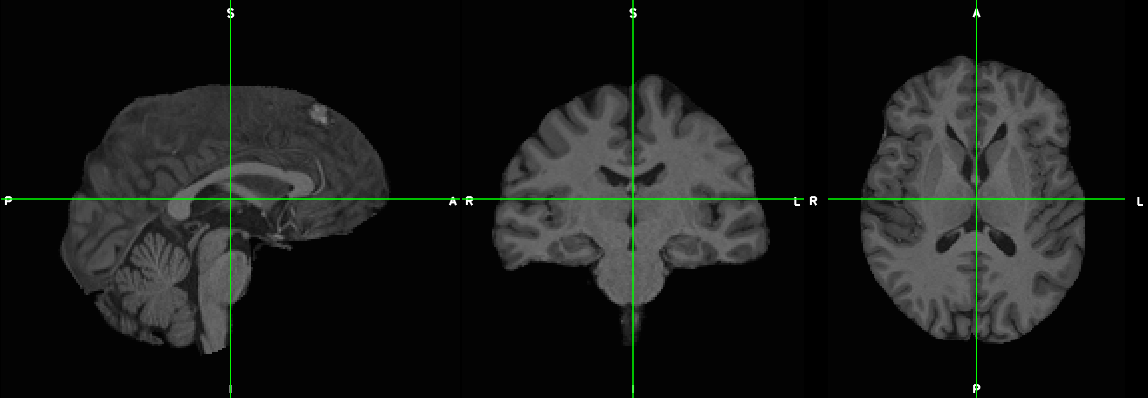
\includegraphics[width=0.6\textwidth]{T1.png}
    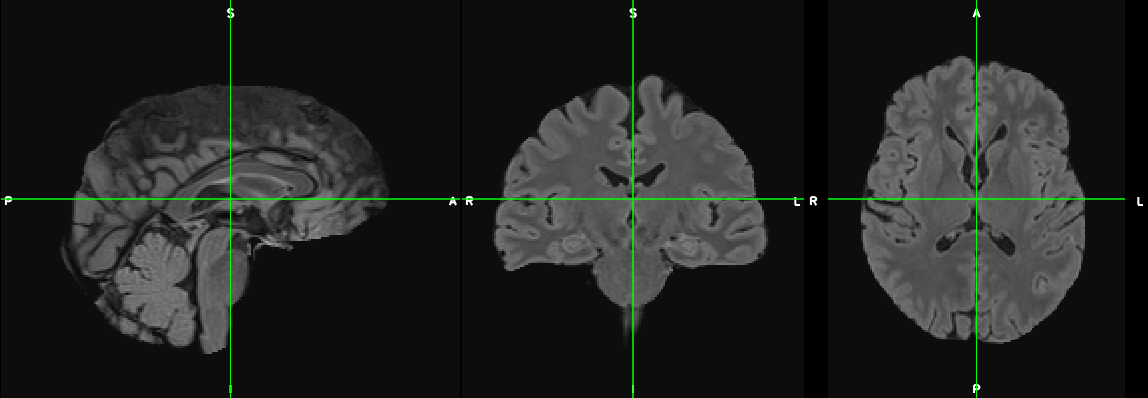
\includegraphics[width=0.6\textwidth]{T2.png}
    \caption{The slices of the T1 (top) T2-weighted FLAIR (bottom) MRI image.}\label{figure:t1-t2}
\end{figure}


\subsection{Functional features}
\label{fmri}

Functional MRI (fMRI) data indirectly measures brain activity over time. It is represented by \textit{blood oxygenation level dependent} (BOLD) time-series (Figure~\ref{figure:fmri}) that show changes in oxygenation of the blood vessels. Sudden increases in oxygen demand are related to higher brain activity in the corresponding brain region.

The two types of an fMRI image are \textit{task} fMRI, when the subject is asked to perform a specific cognitive task, and \textit{resting state} fMRI (rs-fMRI), when the subject is not performing any particular task. This project will use rs-fMRI data.

For the purposes of machine learning analysis, \textit{functional connectivity matrices} will be derived from rs-fMRI and used as input features to the graph neural network models. Functional connectivity is conceptualised as the correlation between the time-series of every pair of brain regions together under the assumption that parts of the brain that have related functions would also have similar activity patterns (highly correlated time-series). 


% As a consequence, we would expect higher correlation between the corresponding BOLD time-series. For time-series $T_1$ and $T_2$, \textit{Pearson's correlation} (denoted as $r$) is computed as

% \begin{equation}
%     r(T_1, T_2) = \frac{\mathrm{cov}(T_1, T_2)}{\sigma_{T_1} \sigma_{T_2}}
% \end{equation}

% where $\mathrm{cov}(\cdot, \cdot)$ denotes covariance and $\sigma$ stands for standard deviation.

% The correlations are used to derive the \textit{functional connectivity matrix} storing pairwise correlations between the different voxels (or parcels) as the overall representation of functional brain connectivity. For time-series $T_1, \dots, T_N$,

% \begin{equation}
%     \mathrm{fcm}(T_1, \dots, T_N) = \begin{bmatrix}
%         r(T_1, T_1) & \cdots & r(T_1, T_N) \\
%         \vdots & \ddots & \vdots \\
%         r(T_N, T_1) & \cdots & r(T_N, T_N)
%     \end{bmatrix},
% \end{equation}

% of which (due to symmetry and the non-informative diagonal) only the flattened lower triangle is usually used as input for the downstream machine learning analysis.


% Could include (Pearson's, lasso, partial correlation, covariance)

% Tiago's observation that partial correlation may give better results when including functional MRI time-series in the machine learning model.
% From wiki on partial correlation: In probability theory and statistics, partial correlation measures the degree of association between two random variables, with the effect of a set of controlling random variables removed. If we are interested in finding whether or to what extent there is a numerical relationship between two variables of interest, using their correlation coefficient will give misleading results if there is another, confounding, variable that is numerically related to both variables of interest. This misleading information can be avoided by controlling for the confounding variable, which is done by computing the partial correlation coefficient. This is precisely the motivation for including other right-side variables in a multiple regression; but while multiple regression gives unbiased results for the effect size, it does not give a numerical value of a measure of the strength of the relationship between the two variables of interest.

\begin{figure}[]
    \centering
    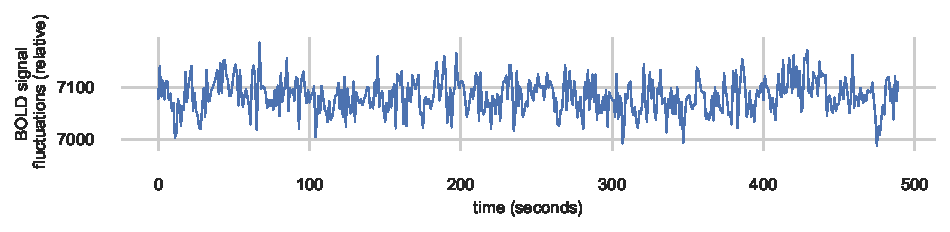
\includegraphics[width=\textwidth]{fmri.pdf}
    \caption{An example of a BOLD time-series for a single brain region.}\label{figure:fmri}
\end{figure}

\subsection{Euler indices}
The Euler index~\cite{rosen2018quantitative} is a quality control metric which represents the number of times the HCP Freesurfer brain reconstruction software failed to seamlessly connect two 2D slices of an MRI image into the 3D representation of the brain. The higher the Euler index, the worse is the quality of the scan. Euler indices might be used to remove the subjects with low-quality scans to avoid them affecting the analysis~\cite{kaufmann2019} (in this project this was not needed because the indices were generally low). Alternatively, Euler indices can be used as a covariate in a machine learning model (as a brain similarity metric or a node feature) to correct for any scan quality-related bias in prediction. This project will use Euler indices as node features for consistency in keeping neuroimaging features in nodes and non-imaging features in edges.


\subsection{Neuroimaging data preprocessing}

All MRI and fMRI data in UKB was preprocessed (denoised and motion-corrected) with standard UK Biobank pipelines\footnote{\url{https://biobank.ctsu.ox.ac.uk/crystal/crystal/docs/brain_mri.pdf}}. For the purpose of this study, the data was further \textit{parcellated} at the Department of Psychiatry by Dr Richard Bethlehem, Dr Rafael Romero-Garcia and Dr Lisa Ronan\footnote{\url{https://github.com/ucam-department-of-psychiatry/UKB}}.

A \textit{parcellation} splits an image of a brain into biologically meaningful regions for downstream analysis, compressing per-voxel\footnote{A \textit{voxel} is a discrete volumetric element.} measurements into per-parcel summaries (see Figure~\ref{figure:parcellated-brain} for an example). In this dissertation, the neuroimaging data will be parcellated with one of the most common parcellations developed by Glasser et al.~\cite{glasser2016multi}, which divides the brain into 360 cortical regions and 16 subcortical regions. 


\begin{figure}[h!]
    \centering
    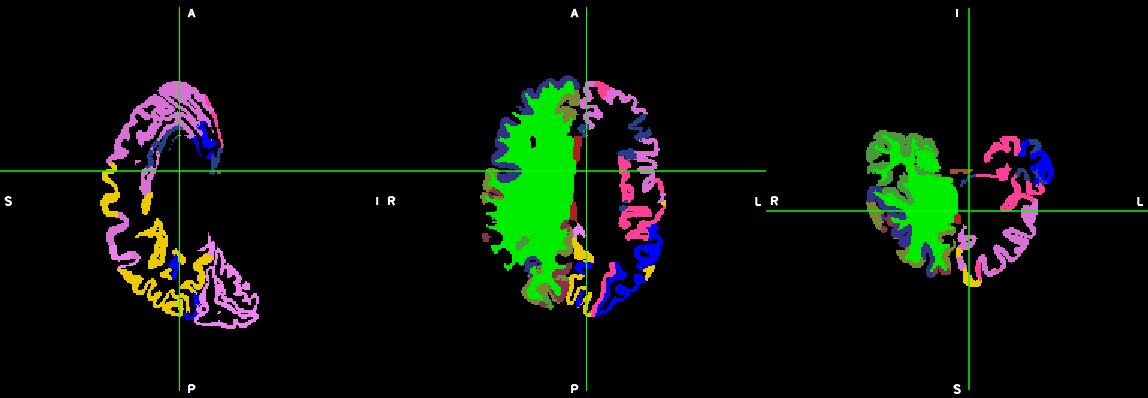
\includegraphics[width=0.6\textwidth]{parcellated_brain.png}
    \caption{The slices of the MRI image with parcels highlighted in different colours.}\label{figure:parcellated-brain}
\end{figure}

% When the brain is imaged there is a choice whether to warp the image of the brain to the fixed atlas or whether to warp the atlas to match the variable brain images. The former makes it easier to process a dataset of many images and find the matching regions of two brains faster, but the latter remains more faithful to the unique structure of the individual patient's brain. 

\subsection{Non-imaging features}

In this dissertation, non-imaging data refers to all subject data that does not come from structural MRI and fMRI scans. The features useful to this project include the subject's binary (biological) sex, the psychiatric disorder diagnoses, mental health status, education, and other variables that might have a confounding effect on structure and functional connectivity of the brain~\cite{ruigrok2014meta} and consequently affect the brain age. Table \ref{table:phenotype-features} summarises the non-imaging features selected for this project.
\stepcounter{footnote}
\begin{table}[h]
    \caption{Summary of the non-imaging features used in this project.}\label{table:phenotype-features}
    \centering
    \begin{tabular}{cp{6cm}p{7.5cm}}
        \hline
    \textbf{Code} & \textbf{Non-imaging feature} & \textbf{Explanation} \\ \hline
    \texttt{AGE} & Chronological age &  Used as the training label. \\
    \texttt{FI} & Fluid intelligence score &  Measures cognitive performance. Related to increased brain activity~\cite{gray2003neural}. \\
    \texttt{FTE} & Years of full-time education &  Associated with brain age gaps~\cite{steffener2016differences} and other brain health conditions~\cite{brayne2010education}.\\
    \texttt{ICD10} & Mental and brain health (from ICD10 diagnosis code data) & Subject mental health and nervous system disease diagnoses that might affect the structure and function of the brain. Diagnoses were grouped by categories following the ICD10 system\footnotemark[\value{footnote}]. \\
    \texttt{MEM} & Prospective memory result & Memory generally declines with age, and is related to changing brain activity patterns~\cite{grady2000changes, kliegel2006delayed}. \\
    \texttt{SEX} & Binary sex (male or female) & Highly affects the size and volume of the brain~\cite{ruigrok2014meta}. \\ \hline
    \end{tabular}
\end{table}
\footnotetext[\value{footnote}]{\url{https://icd.who.int/browse10/2019/en}}
\stepcounter{footnote}

The non-imaging data is used to compute the inter-subject similarity score, which will determine the edges of the population graph.

\section{Population graphs}
\label{population-graphs}

One useful way to combine the multiple types of neuroimaging data and represent the relations between subjects for downstream machine learning tasks is a \textit{population graph} data structure, as it is presented by Parisot et al.~\cite{parisot2018disease}.

The set of $N$ subjects $S$ is connected into an undirected population graph $G = (V, E)$, where $V$ is the set of graph nodes (with one node uniquely representing one subject), and $E$ is the set of edges (representing the similarity of subjects).

Each node $v \in V$ is a vector containing the individual subject's neuroimaging data, whether structural, functional, or both. The edge $(v, w) \in E$ connects subjects $s_v, s_w \in S$ based on some \textit{similarity metric} that uses the non-imaging information of the subjects to create edges between the nodes. 

Defining a good similarity metric is important to account for the confounding effects on the feature vectors (e.g. the subject's sex affects the brain volume) as well as to cluster subjects into the most informative neighbourhoods. For example, in this dissertation the neighbourhoods that have similar brain age gaps could be useful. If carefully defined, the similarity metrics could include the domain expertise of neurologists and psychiatrists as well.

Similarity metrics are defined using a \textit{similarity function} $\mathrm{sim}(\cdot, \cdot)$ which takes two subjects and returns the similarity score between them (the higher the score, the more similar are the subjects):

\begin{equation}
    \mathrm{sim}(s_v, s_w) = \frac{1}{n}\sum_{i=1}^{n} \mathbf{1}[M_i(s_v) = M_i(s_w)].
    \label{eq:similarity}
\end{equation}

Here $\{M_1, \dots, M_n\}$ is a set of non-imaging features that are used to compute subject similarity and $\mathbf{1}[\cdot]$ is an indicator function, in this case returning a non-zero value when the values for a given non-imaging feature $M_i$ match for the two subjects $s_v$ and $s_w$. In practice, if the metric is a real number, ``matching'' could be defined in terms of non-imaging features being within some constant $\epsilon > 0$. 

To avoid memory issues when $|E| \sim O(N^2)$ and minimise the size of the neighbourhood to only highly similar subjects, a \textit{similarity threshold} $\mu$ is used such that

\begin{equation}
    (v, w) \in E \iff \mathrm{sim}(s_v, s_w) \geq \mu.
    \label{eq:similarity-threshold}
\end{equation}

The population graphs can only be effectively accepted as input to machine learning models that are capable of operating on graph-structured data. The two following sections will discuss two types of \textit{graph neural networks} (GNNs) that will be implemented in this dissertation for this purpose, namely graph convolutional and graph attention networks.

\section{Graph convolutional networks}
\label{training-gcn}
% What is actually essential about the graph convolutional networks?

One of the approaches of how the graphs can be represented in neural networks is based on spectral graph theory~\cite{hammond2011wavelets}. The main advantage of this strategy is that it makes the operations applied to every node independent of the local graph topology (the number of neighbours of a particular node). This is easier to optimise as the same operation can be applied to all nodes. 

The graph is therefore first transformed from spatial (Euclidean) to spectral (Fourier) domain. The more expensive convolution operation in the Euclidean domain corresponds to a cheaper multiplication operation in the Fourier domain.

\subsection{Graph spectral decomposition}

In spectral analysis, a graph $G = (V, E)$ is represented by its \textit{normalised graph Laplacian} matrix~\cite{defferrard2016convolutional}: 

\begin{equation}
    \mathbf{L} = \mathbf{I} - \mathbf{D}^{-1/2}\mathbf{A}\mathbf{D}^{-1/2},
\end{equation}

where $\mathbf{I}$ is the identity matrix, $\mathbf{D} \in \mathbb{N}^{N \times N}$ is the diagonal degree matrix of the graph nodes, and $\mathbf{A} \in \{0, 1\}^{N \times N}$ is the adjacency matrix such that $a_{ij} = \mathbf{1}[(i, j) \in E]$. The graph Laplacian uniquely represents the graph as it is based on the graph's topology.

The positive semidefinite graph Laplacian matrix is decomposed as

\begin{equation}
    \mathbf{L} = \mathbf{U\Lambda U}^\mathrm{T},
\end{equation}

where $\mathbf{\Lambda}$ is the diagonal eigenvalue matrix, and $\mathbf{U}$ is the eigenbasis defining the graph Fourier domain: for a signal $\mathbf{x} \in \mathbb{R}^{F}$ (e.g. a graph node with $F$ features), $\mathbf{\hat{x}} = \mathbf{U}^\mathrm{T}\mathbf{x}$ is the \textit{graph Fourier transform} of $\mathbf{x}$, and $\mathbf{x} = \mathbf{U}\mathbf{\hat{x}}$ is its inverse~\cite{wu2019simplifying}.

% Eigenvalues as graph frequencies and learning as a low-pass filter of frequencies.
% Fourier transform as transformation to the eigenbasis obtained through graph Laplacian diagonalisation.

%~\cite{velickovic2018graph}: graph definition in the Fourier domain based on the eigendecomposition of the graph Laplacian

\subsection{Spectral graph convolution}

For a filter $\mathbf{g} \in \mathbb{R}^m$ with a diagonal matrix $\mathbf{\hat{G}} = \mathrm{diag}(\mathbf{U}^\mathrm{T}\mathbf{g})$ containing the filter's spectral coefficients, the graph convolution of a signal $\mathbf{x}$ is defined as

\begin{equation}
    \label{eq:convolution}
    \mathbf{x} *_G \mathbf{g} = \mathbf{U}((\mathbf{U}^\mathrm{T}\mathbf{x}) \odot (\mathbf{U}^\mathrm{T}\mathbf{g})) = \mathbf{U}\mathbf{\hat{G}}\mathbf{U}^\mathrm{T}\mathbf{x}
\end{equation}

where $\odot$ is the element-wise (Hadamard) product~\cite{wu2019simplifying}.

\subsection{Optimising graph convolutions}
This section reviews the steps towards optimised graph convolutional networks (GCNs) as proposed by Kipf and Welling~\cite{kipf2017semi}.

\subsubsection{ChebNets}
To avoid the $O(N^2)$ filtering operation due to the matrix-vector multiplications in Equation~\eqref{eq:convolution}, Defferrard et al.'s~\cite{defferrard2016convolutional} ChebNets use recursively defined \textit{Chebyshev polynomials}

\begin{gather}
    T_k(\mathbf{M}) = 2\mathbf{M}T_{k-1}(\mathbf{M}) - T_{k-2}(\mathbf{M}) \\
    T_1 = \mathbf{M} \\
    T_0 = \mathbf{I}
\end{gather}

to approximate the filter $\mathbf{\hat{G}}$ as 

\begin{equation}
    \mathbf{\hat{G}} \approx \sum_{k = 0}^{K} \theta_k T_k(\mathbf{\tilde{\Lambda}})
\end{equation}

where $\mathbf{\tilde{\Lambda}} = 2\mathbf{\Lambda}/\lambda_{\mathrm{max}} - \mathbf{I}$, $\lambda_\mathrm{max}$ is the largest eigenvalue in $\mathbf{\Lambda}$, and $\theta_k$ are coefficients such that $\mathbf{\hat{G}} = \sum_k \theta_k \mathbf{\Lambda}^k$~\cite{wu2019simplifying}. The truncation coefficient (polynomial order) $K$ corresponds to the neighbourhood of at most $K$ hops away from the node of interest, and such convolution is said to be $K$-localised. 

Next, it can be proved~\cite{wu2019comprehensive} that

\begin{equation}
    T_k(\mathbf{\tilde{L}}) = \mathbf{U}T_k(\mathbf{\tilde{\Lambda}})\mathbf{U}^{\mathrm{T}}
\end{equation}

with $\mathbf{\tilde{L}} = 2\mathbf{L}/\lambda_{\mathrm{max}} - \mathbf{I}$. The result is the approximated spectral graph convolution:

\begin{equation}
    \label{eq:chebnet}
    \mathbf{x} *_G \mathbf{g} \approx \sum_{k=0}^{K}\theta_k T_k(\mathbf{\tilde{L}})\mathbf{x}.
\end{equation}

% ChebNet: filters further approximated by Chebyshev expansion of the graph Laplacian avoiding the expensive eigendecomposition operation (ChebNet) (velickovic)

\subsubsection{GCNs}
Kipf and Welling's GCNs~\cite{kipf2017semi} introduce further optimisations to ChebNets: 
\begin{enumerate}
    \item Taking $K=1$ makes Equation~\eqref{eq:chebnet} linear, which is more suitable for neural network architectures with linear layers and non-linearities between them.
    \item To minimise the number of trainable parameters, $\theta_0$ and $\theta_1$ become functions of a single parameter $\theta$: $\theta = \theta_0 = -\theta_1$.
    \item Further assuming $\lambda_{\mathrm{max}}\approx 2$ simplifies the computation of $\mathbf{\tilde{L}}$, since this eliminates the need for eigendecomposition of the Laplacian: $\mathbf{\tilde{L}} = 2\mathbf{L}/\lambda_{\mathrm{max}} - \mathbf{I}$ becomes $\mathbf{\tilde{L}} \approx \mathbf{L} - \mathbf{I}$.
\end{enumerate}

This results in convolution approximation:

\begin{align}
    \mathbf{x} *_G \mathbf{g} &\approx \theta_0 T_0(\mathbf{\tilde{L}}) \mathbf{x} + \theta_1 T_1(\mathbf{\tilde{L}}) \mathbf{x} \\
    &\approx \theta \mathbf{I} \mathbf{x} - \theta (\mathbf{L} - \mathbf{I}) \mathbf{x} \\
    \label{eq:gcnconv1}
    &= \theta(\mathbf{I} + \mathbf{D}^{-1/2}\mathbf{A}\mathbf{D}^{-1/2})\mathbf{x}
\end{align}

Finally, to avoid the numerical instability of repeated convolutions due to the eigenvalues of the matrix in Equation~\eqref{eq:gcnconv1} ranging in $[0, 2]$, a \textit{renormalisation trick} is applied by adding self-loops to the graph nodes: taking $\mathbf{\tilde{A}} = \mathbf{A} + \mathbf{I}$ and $\mathbf{\tilde{D}}$ the degree matrix of $\mathbf{\tilde{A}}$, 

\begin{equation}
    \label{eq:gcnconv2}
    \mathbf{x} *_G \mathbf{g} \approx \theta(\mathbf{\tilde{D}}^{-1/2}\mathbf{\tilde{A}}\mathbf{\tilde{D}}^{-1/2})\mathbf{x}.
\end{equation}
 
% (this citation also very good for follow through for what the training is doing for all layers in general rather than a single feature vector, i.e. the training flow)
% can also mention~\cite{wu2019comprehensive};

% extension: an alternative to Chebyshev polynomials (extension): cayleynet--probably too difficult to implement

\subsection{Graph convolutional layer}
The graph convolution operation in Equation~(\ref{eq:gcnconv2}) is generalised to the entire layer of the network as follows. 

Let $\mathbf{H}^{(l-1)} \in \mathbb{R}^{N\times C_{l-1}}$ be the input layer of a neural network with $C_{l-1}$ input channels, $\mathbf{H}^{(l)} \in \mathbb{R}^{N\times C_{l}}$ be the GCN layer with $C_{l}$ output channels, and $\mathbf{H}^{(0)} = \mathbf{X} \in \mathbb{R}^{N \times C_0}$ containing $C_0$ input features for each of the $N$ nodes in the population graph (in this case the neuroimaging data for $N$ subjects). For the weight matrix $\mathbf{\Theta}^{(l)} \in \mathbb{R}^{C_{l-1}\times C_{l}}$ and an activation function $\sigma(\cdot)$,

\begin{equation}
    \mathbf{H}^{(l)} \leftarrow \sigma( \mathbf{\tilde{D}}^{-1/2}\mathbf{\tilde{A}}\mathbf{\tilde{D}}^{-1/2}\mathbf{H}^{(l-1)}\mathbf{\Theta}^{(l)}).
\end{equation}

\section{Graph attention networks}
\label{training-gat}

In contrast to the \textit{spectral} GCN that relies on the computation within the Fourier domain using the graph Laplacian, the graph attention network (GAT)~\cite{velickovic2018graph} is a \textit{spatial} architecture that operates in the Euclidean domain. Here, the mechanism that incorporates the neighbourhood information is defined to work on the neighbourhoods of different sizes, with each node learning how much importance (\textit{attention}) it should assign to each one of its neighbours.

% \textit{Self-attention} is also added in to the concept where different parts of the node's neighbourhood are considered with different importance weights, getting a representation of the rest of the neighbourhood. 

\subsection{Graph attentional layer}
Analogously to the previous section, we consider an input layer $\mathbf{H}^{(l-1)} \in \mathbb{R}^{N\times C_{l-1}}$ (with $\mathbf{H}^{(0)} = \mathbf{X} \in \mathbb{R}^{N\times C_{0}}$ as before) and the GAT layer $\mathbf{H}^{(l)} \in \mathbb{R}^{N\times C_{l}}$. Denote the input layer $\mathbf{H}^{(l-1)}$ as $[\mathbf{h}_1^{(l-1)} \cdots \mathbf{h}_{N}^{(l-1)}]^{\mathrm{T}}$, and $\mathbf{H}^{(l)}$ as $[\mathbf{h}_1^{(l)} \cdots \mathbf{h}_{N}^{(l)}]^{\mathrm{T}}$. For a trainable weight matrix $\mathbf{W}^{(l)} \in \mathbb{R}^{C_{l} \times C_{l-1}}$ and an \textit{attentional mechanism} $a: \mathbb{R}^{C_{l}} \times \mathbb{R}^{C_{l}} \rightarrow \mathbb{R}$ we compute (unnormalised) \textit{attentional coefficients} $e_{ij}$:

\begin{equation}
    e_{ij} = a(\mathbf{W}^{(l)}\mathbf{h}_i^{(l-1)}, \mathbf{W}^{(l)}\mathbf{h}_j^{(l-1)}).
\end{equation}

In Veli{\v{c}}kovi\'{c} et al.~\cite{velickovic2018graph}, the attention mechanism is implemented as a linear transformation using a learnable weight vector $\mathbf{a} \in \mathbb{R}^{2C_{l}}$, followed by a non-linearity $\mathrm{LeakyReLU}(\cdot)$ with slope 0.2 for negative input:

\begin{align}
    e_{ij} &= a(\mathbf{W}^{(l)}\mathbf{h}_i^{(l-1)}, \mathbf{W}^{(k)}\mathbf{h}_j^{(l-1)}) \\
    &= \mathrm{LeakyReLU}(\mathbf{a}^{\mathrm{T}}[\mathbf{W}^{(l)}\mathbf{h}_i^{(l-1)} \parallel \mathbf{W}^{(l)}\mathbf{h}_j^{(l-1)}]),
\end{align}

where $\parallel$ denotes concatenation.

The graph topology is accounted for by discarding any coefficients $e_{ij}$ where $(i, j) \notin E$, and normalising the coefficients $\alpha_{ij}, (i, j) \in E$ for the rest using the softmax function:

\begin{align}
    \alpha_{ij} &= \underset{{j: (i, j) \in E}}{\mathrm{softmax}}\left(e_{ij}\right) \\
    &= \underset{{j: (i, j) \in E}}{\mathrm{softmax}}\left(\mathrm{LeakyReLU}(\mathbf{a}^{\mathrm{T}}[\mathbf{W}^{(l)}\mathbf{h}_i^{(l-1)} \parallel \mathbf{W}^{(l)}\mathbf{h}_j^{(l-1)}])\right) \\
    &=  \frac{\mathrm{exp}\left(\mathrm{LeakyReLU}(\mathbf{a}^{\mathrm{T}}[\mathbf{W}\mathbf{h}_i^{(l-1)} \parallel \mathbf{W}^{(l)}\mathbf{h}_j^{(l-1)}])\right)}{\sum\limits_{k: (i, k) \in E}\mathrm{exp}\left(\mathrm{LeakyReLU}(\mathbf{a}^{\mathrm{T}}[\mathbf{W}^{(l)}\mathbf{h}_i^{(l-1)} \parallel \mathbf{W}^{(l)}\mathbf{h}_k^{(l-1)}])\right)}.
\end{align}

The coefficients $\alpha_{ij}$ and the weight matrix are used to compute the output features for another non-linearity $\sigma$:

\begin{equation}
    \label{eq:attention}
    \mathbf{h}_i^{(l)} = \sigma\left(\sum\limits_{j: (i, j) \in E} \alpha_{ij}\mathbf{W}^{(l)}\mathbf{h}_j^{(l-1)}\right)
\end{equation}

\subsection{Multi-head attention}
The above attention mechanism can be repeated several times to stabilise the performance, where one independent application of attention is called an \textit{attention head}. The outputs of the independent attention heads are concatenated or averaged together until the last layer of the complete neural network architecture when they are averaged into a single output. For $M$ attention heads, the results of Equation~\eqref{eq:attention} are concatenated in non-final layers:

\begin{equation}
    \mathbf{h}_i^{(l)} = \underset{m=1}{\overset{M}{\big\|}} \sigma\left(\sum\limits_{j: (i,j)\in E} \alpha_{ij, m}\mathbf{W}^{(l)}_m\mathbf{h}_j^{(l-1)}\right),
\end{equation}

or averaged if GAT is the final ($L$-th) layer of the network:

\begin{equation}
    \mathbf{h}_i^{(L)} = \sigma\left(\frac{1}{M}\sum\limits_{m=1}^M\sum\limits_{j: (i,j)\in E} \alpha_{ij, m}\mathbf{W}^{(L)}_m\mathbf{h}_j^{(L-1)}\right).
\end{equation}

\section{Training task}
\label{training-task}
% Train/validation/test split, cross-validation, patient selection and exclusion from results, stratification, graph representation (edge lists, node features, edge features,...)

% Labels are available for a small subset of nodes and are spread across neighbourhoods through a regularisation term such as Laplacian~\cite{kipf2017semi}, predicting the labels for the remaining nodes

For node label prediction tasks such as brain age estimation, the population graphs are trained in a \textit{semi-supervised} manner: while the entire dataset (every node and edge) is included in the graph, only a subset of the nodes is labelled, with the goal being to learn the labels for the remaining nodes~\cite{kipf2017semi}. At each training step (epoch), the feedback from nodes with available labels is used to update the parameters for the entire graph, which could be seen as information being ``propagated'' from a labelled node to the neighbours that are similar to it (as defined by the similarity metric). After the model is trained, every node in the population graph has a prediction for its label.

The predictive power of a model can be evaluated based on its performance on a set of test nodes, for which the labels had been invisible to the model at the training stage. For the brain age estimation task, the metrics used to evaluate the performance are Pearson's correlation $r$ and coefficient of determination $r^2$~\cite{niu2019improved}.


% TODO \textit{an illustration of the graph with marked training and validation nodes with visible labels and how the training happens on those followed by how the graph is evaluated on the test nodes where the parameters were updated but the labels never seen} – maybe include in GCN/GAT sections instead?

% TODO illustrations could also explain the operation of the networks, perhaps highlighting differences between GCN and GAT graphically: Averaging representations of neighbour features and smoothing labels as a consequence.~\cite{wu2019simplifying}


\section{Requirements analysis}
\label{section:requirements-analysis}

The project has three main stages that directly correspond to the Success Criteria of the Project Proposal (Appendix~\ref{chapter:project-proposal}):

\begin{enumerate}[label=S\arabic*.]
    \item Implementation of the population graph data structure, with nodes containing the individual neuroimaging data and edges representing associations between them based on pairwise similarity. This involves: \begin{enumerate}[label=\theenumi\arabic*.]
        \item Preprocessing of the functional, structural imaging and non-imaging data of the UKB subjects.
        \item Implementation of the similarity functions that would compare two subjects and return similarity scores in increasingly flexible manner: the basic function as defined in Equation~\eqref{eq:similarity}, and extensions for accepting any linear combinations of similarity features and arbitrary similarity functions.
        % TODO RB: For when you have more time we can think further about how to optimise that by perhaps including more measures. Not for now though :)
        \item A pipeline that would generate the population graph for a given set of subjects, their modalities, similarity metric and similarity threshold.
        % An extension for supporting higher flexibility in similarity metrics by including the similarity score as an edge feature rather than having a 1-weighted edge whenever the similarity score exceeds a given threshold
    \end{enumerate}
    \item Implementation of the graph convolutional network (GCN) and graph attention network (GAT) architectures for the age regression task. 
    \item Training and evaluation of the two graph neural network architectures on the UKB population graph. This includes the extension of implementing the robustness measurement framework.
\end{enumerate}

I expect stage S1 to be the most complex for the following additional requirements.
\begin{enumerate}[label=R\arabic*.]
    \item Care must be taken to make sure that the data is handled \textit{correctly}. This will require testing of the components which transform the data to the population graph data structure.
    \item The pipeline must be \textit{flexible} enough to support the various combinations of modalities, subjects, and similarity metrics, which will be ensured by independent support of every modality and the \textit{extension} of the project to support custom similarity functions.
    \item The pipeline has to be \textit{modular} enough to be easily extended to more datasets, modalities and processing options in the future. To achieve this, the pipeline will be split into independent components with their own designated functionality, so that they are easier to build upon independently.
\end{enumerate} 

These considerations by themselves largely fulfil the proposed \textit{extension} of implementing the pipeline that can handle raw data at the one of its earliest processing stages in an end-to-end manner – indeed any earlier stage would require advanced neuroimaging processing expertise that would be out of scope of a Computer Science Part II project. 

The full design of the neuroimaging processing pipeline with respect to those requirements, as well as the GCN and GAT architectures and their evaluation, is discussed in Chapter~\ref{chapter:implementation}.

\section{Software engineering practice}
Since every stage discussed in the previous section depends on the implementation of the stage before it, the straightforward workflow is to carry out the three stages in order (except for the extensions, which would be implemented last). This fits best with the \textit{waterfall model} of software development because the project is relatively small and has a straightforward set of requirements, the design of the pipeline directly corresponds to the three project stages, and implementation depends on how the different pipeline stages are designed to interact with each other. Chapter~\ref{chapter:implementation} walks through the schematic design diagrams that were used as foundation for the component implementation.

To track the workflow, prevent loss of data and ease the readability and/or any future extensions to this project, the common practices of consistent code style (adhering to PEP8\footnote{\url{https://www.python.org/dev/peps/pep-0008/}} style guide), comprehensive documentation, unit testing, code reuse, version control (through a \texttt{git} repository), and backup strategies (regular backups to an external disk, GitHub repository, and Google Drive) will be applied.

\section{Choice of tools}

Because of its popularity and wide community support in both machine learning and neuroimaging, I chose Python as the implementation language for this interdisciplinary project.

This project will use \textit{PyTorch Geometric}~\cite{fey2019pytorch}, a popular extension library for \textit{PyTorch}~\cite{pytorch} that provides out-of-the-box graph neural network architecture implementations and has the advantage over other libraries (and other machine learning frameworks such as TensorFlow) of being easy to learn and use. 

The neuroimaging machine learning library \textit{Nilearn} will be used for some of the neuroimaging data processing and visualisation~\cite{abraham2014machine, nilearn}.

For scientific computing, I will use common Python packages such as \textit{scikit-learn}~\cite{pedregosa2011scikit}, \textit{pandas}~\cite{mckinney2010scipy}, and \textit{NumPy}~\cite{walt2011numpy}. 

For testing, I will use Python's \texttt{unittest} library.

For model logging, visualisation and hyperparameter tuning, I will use the free \textit{Weights~\& Biases}~\cite{wandb} framework because of its clean, intuitive interface and automated machine learning capabilities.


\section{Starting point}
The discussion of the architectures proposed in this section assumes or uses the knowledge of the Computer Science Tripos courses: IA NST Mathematics, IA Scientific Computing, IA Machine Learning and Real-world Data, IB Foundations of Data Science, IB Artificial Intelligence, II Data Science: Principles and Practice, II Machine Learning and Bayesian Inference. The conceptual understanding of the brain age estimation, neuroimaging data processing and graph neural networks (none of which I had previous experience with) required the study of papers cited as well as other supporting resources.

The code builds on implementations provided by the packages listed in the previous section. I had no previous experience with most of them.

The preprocessed dataset has been provided by Dr Richard Bethlehem of Department of Psychiatry.